\vspace{-1.5em}
\section{Shortest Path}
\begin{theo}[Dijkstra's Algorithm]
    
    \textbf{Proposition:} Suppose that there is a shortest path from nodes $u\to v$. Then any
    sub-path between these nodes, say $x\to y$, is also the shortest path.\\

    \noindent
    \textbf{Algorithm:} Given a weighted graph $G$ and a source node $s$, 
    \begin{enumerate}
        \item [(i.)] Keep track of best distances, start at a queue with $s$.
        \item [(ii.)] Pop off the queue, flag item as visited.
        \item [(iii.)] View all children weights, update if it's the new shortest path to that node.
        \item [(iv.)] Queue children in ascending order of weight (smallest$\to$largest)
    \end{enumerate}
    Preform steps (ii) to (iv) until the queue is empty, having visited all possible nodes.
\end{theo}


\vspace{-1em}
\begin{Proof}[Proof of Correctness for Dijkstra's Algorithm]

    \textbf{Invariant:} For each node $u \in S$, $d(u)$ is length of shortest path $s \leadsto u$. By induction on $|S|$:\\
    \textbf{Base case:} $|S| = 1$ is true since $S = \{s\}$ and $d(s) = 0$.\\
    \textbf{Inductive hypothesis:} Assume true for $|S| = k \geq 1$.
    \begin{itemize}
        \item Let $v$ be the next node added to $S$, and let $(u, v)$ be the final edge.
        \item A shortest $s \leadsto u$ path plus $(u, v)$ is an $s \leadsto v$ path of length $\pi(v)$.
        \item Consider any $s \leadsto v$ path $P$. We show that it is no shorter than $\pi(v)$.
        \item Let $(x, y)$ be the first edge in $P$ that leaves $S$, and let $P'$ be the subpath to $x$.
        \item $P$ is already too long as soon as it reaches $y$.
    \end{itemize}
    \[
    \ell(P) \geq \ell(P') + \ell(x, y) \geq d(x) + \ell(x, y) \geq \pi(y) \geq \pi(v)
    \]
    \end{Proof}
    
\newpage

\noindent
To visualize our proof consider paths the following diagram:
\begin{figure}[h]
    \begin{center}
      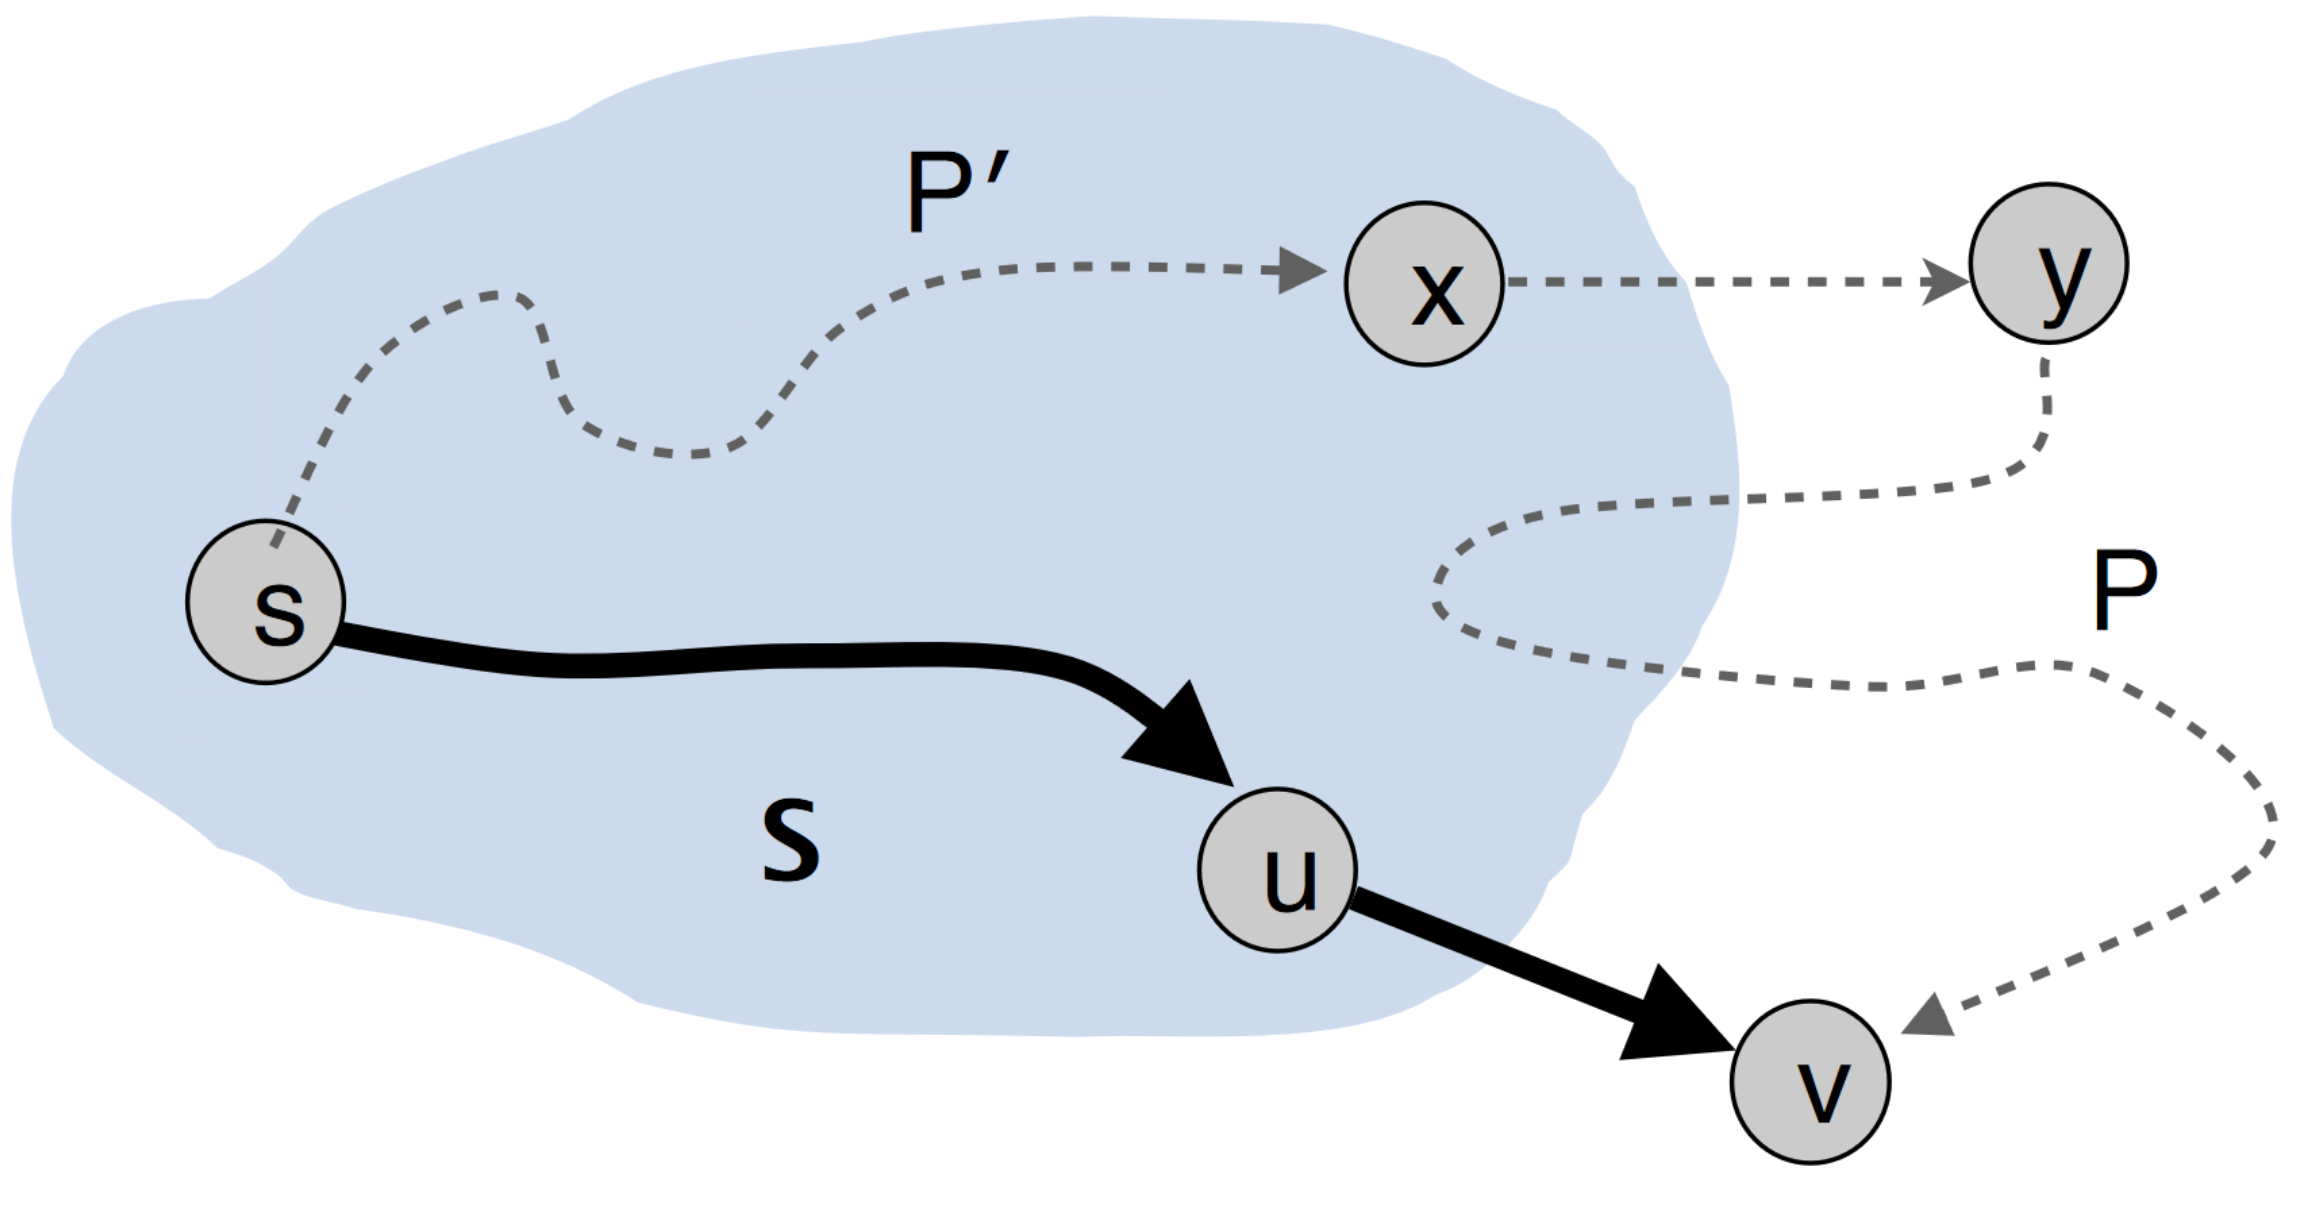
\includegraphics[height=1.3in]{./Sections/dstra/dstra_proof.png}
    \end{center}
     \caption{A system of subset paths (blue), and an exact point of exit $u\to v$ and $x\to y$}\label{fig:dstra_proof}
\end{figure}

\noindent
Since $u\to y$ and $x\to y$ are at the same exact point of exit, i.e., say $s\to v\cong s\to y$, then to go from $y\to v$ must take some additional step.
Therefore, $s\to y\to v$ is longer. \textbf{E.g:} Let $s\to y:= 3$ and $s\to v:= 3$, and all steps take $1$.
Then $s\to y\to v = 4$, while $s\to v = 3$. Therefore $s\to v$ is the shortest path.\\

\noindent
\textbf{Dijkstra Example (i):} To emphasize the BFS nature of Dijkstra's algorithm:
\begin{figure}[h]
    
    \centering
    \tikzset{every picture/.style={line width=0.75pt}} %set default line width to 0.75pt        

    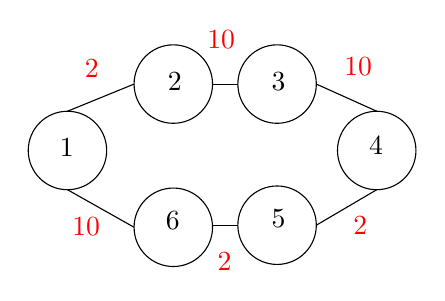
\begin{tikzpicture}[x=0.75pt,y=0.75pt,yscale=-1,xscale=1]
    %uncomment if require: \path (0,300); %set diagram left start at 0, and has height of 300

    %Shape: Circle [id:dp7522181001310076] 
    \draw   (171,142.9) .. controls (171,132.46) and (179.46,124) .. (189.9,124) .. controls (200.34,124) and (208.8,132.46) .. (208.8,142.9) .. controls (208.8,153.34) and (200.34,161.8) .. (189.9,161.8) .. controls (179.46,161.8) and (171,153.34) .. (171,142.9) -- cycle ;
    %Shape: Circle [id:dp46823217732954925] 
    \draw   (222,179.9) .. controls (222,169.46) and (230.46,161) .. (240.9,161) .. controls (251.34,161) and (259.8,169.46) .. (259.8,179.9) .. controls (259.8,190.34) and (251.34,198.8) .. (240.9,198.8) .. controls (230.46,198.8) and (222,190.34) .. (222,179.9) -- cycle ;
    %Shape: Circle [id:dp7637679019155722] 
    \draw   (222,110.9) .. controls (222,100.46) and (230.46,92) .. (240.9,92) .. controls (251.34,92) and (259.8,100.46) .. (259.8,110.9) .. controls (259.8,121.34) and (251.34,129.8) .. (240.9,129.8) .. controls (230.46,129.8) and (222,121.34) .. (222,110.9) -- cycle ;
    %Shape: Circle [id:dp70217655069576] 
    \draw   (272,178.9) .. controls (272,168.46) and (280.46,160) .. (290.9,160) .. controls (301.34,160) and (309.8,168.46) .. (309.8,178.9) .. controls (309.8,189.34) and (301.34,197.8) .. (290.9,197.8) .. controls (280.46,197.8) and (272,189.34) .. (272,178.9) -- cycle ;
    %Shape: Circle [id:dp2788867666411141] 
    \draw   (272,110.9) .. controls (272,100.46) and (280.46,92) .. (290.9,92) .. controls (301.34,92) and (309.8,100.46) .. (309.8,110.9) .. controls (309.8,121.34) and (301.34,129.8) .. (290.9,129.8) .. controls (280.46,129.8) and (272,121.34) .. (272,110.9) -- cycle ;
    %Shape: Circle [id:dp7250177070917547] 
    \draw   (320,142.9) .. controls (320,132.46) and (328.46,124) .. (338.9,124) .. controls (349.34,124) and (357.8,132.46) .. (357.8,142.9) .. controls (357.8,153.34) and (349.34,161.8) .. (338.9,161.8) .. controls (328.46,161.8) and (320,153.34) .. (320,142.9) -- cycle ;
    %Straight Lines [id:da06991122166773422] 
    \draw    (222,110.9) -- (189.9,124) ;
    %Straight Lines [id:da17655964402262492] 
    \draw    (222,179.9) -- (189.9,161.8) ;
    %Straight Lines [id:da8882356134150406] 
    \draw    (259.8,110.9) -- (272,110.9) ;
    %Straight Lines [id:da06318270683409766] 
    \draw    (259.8,178.9) -- (272,178.9) ;
    %Straight Lines [id:da3005609764749789] 
    \draw    (309.8,178.9) -- (338.9,161.8) ;
    %Straight Lines [id:da8117715540109972] 
    \draw    (309.8,110.9) -- (338.9,124) ;

    % Text Node
    \draw (185,136) node [anchor=north west][inner sep=0.75pt]   [align=left] {1};
    % Text Node
    \draw (237,104) node [anchor=north west][inner sep=0.75pt]   [align=left] {2};
    % Text Node
    \draw (287,104) node [anchor=north west][inner sep=0.75pt]   [align=left] {3};
    % Text Node
    \draw (334,135) node [anchor=north west][inner sep=0.75pt]   [align=left] {4};
    % Text Node
    \draw (287,170) node [anchor=north west][inner sep=0.75pt]   [align=left] {5};
    % Text Node
    \draw (236,171) node [anchor=north west][inner sep=0.75pt]   [align=left] {6};
    % Text Node
    \draw (256,84) node [anchor=north west][inner sep=0.75pt]   [align=left] {\textcolor[rgb]{1,0,0}{10}};
    % Text Node
    \draw (322,97) node [anchor=north west][inner sep=0.75pt]   [align=left] {\textcolor[rgb]{1,0,0}{10}};
    % Text Node
    \draw (197,98) node [anchor=north west][inner sep=0.75pt]   [align=left] {\textcolor[rgb]{1,0,0}{2}};
    % Text Node
    \draw (191,174) node [anchor=north west][inner sep=0.75pt]   [align=left] {\textcolor[rgb]{1,0,0}{10}};
    % Text Node
    \draw (261,191) node [anchor=north west][inner sep=0.75pt]   [align=left] {\textcolor[rgb]{1,0,0}{2}};
    % Text Node
    \draw (326.35,173.35) node [anchor=north west][inner sep=0.75pt]   [align=left] {\textcolor[rgb]{1,0,0}{2}};


    \end{tikzpicture}

     \caption{A weighted graph.}\label{fig:dstra_ex1}
\end{figure}

\vspace{-.5em}
\noindent
Where iterations and the queue look like:

\vspace{-1em}
$$\begin{matrix} \text{Iteration Init}&\text{from 1} & \text{from 2} & \text{from 6}&\text{from 3}&\text{from 5}\\ 1:0&1:0&1:0&1:0&1:0&1:0\\ 2:\infty&\textcolor{red}{2:2}&2:2&2:2&2:2&2:2\\ 3:\infty&3:\infty&\textcolor{red}{3:12}&3:12&3:12&3:12\\ 4:\infty&4:\infty&4:\infty&4:\infty&\textcolor{red}{4:22}&\textcolor{red}{4:14}\\ 5:\infty&5:\infty&5:\infty&\textcolor{red}{5:12}&5:12&5:12\\ 6:\infty&\textcolor{red}{6:10}&6:10&6:10&6:10&6:10\\ \end{matrix} $$
$$\begin{matrix} \text{Queue Init}&\text{from 1} & \text{from 2} & \text{from 6}&\text{from 3}&\text{from 5}\\ [1]&[2,6]&[6,3]&[3,5]&[5,4]&[4] \end{matrix}$$

\noindent
Finally visiting 4 to see 3 and 5 have already been visited, ending the algorithm as the queue's empty.


\newpage

\noindent
\textbf{Dijkstra Example (ii):}\\

\begin{figure}[h!]
    \centering
    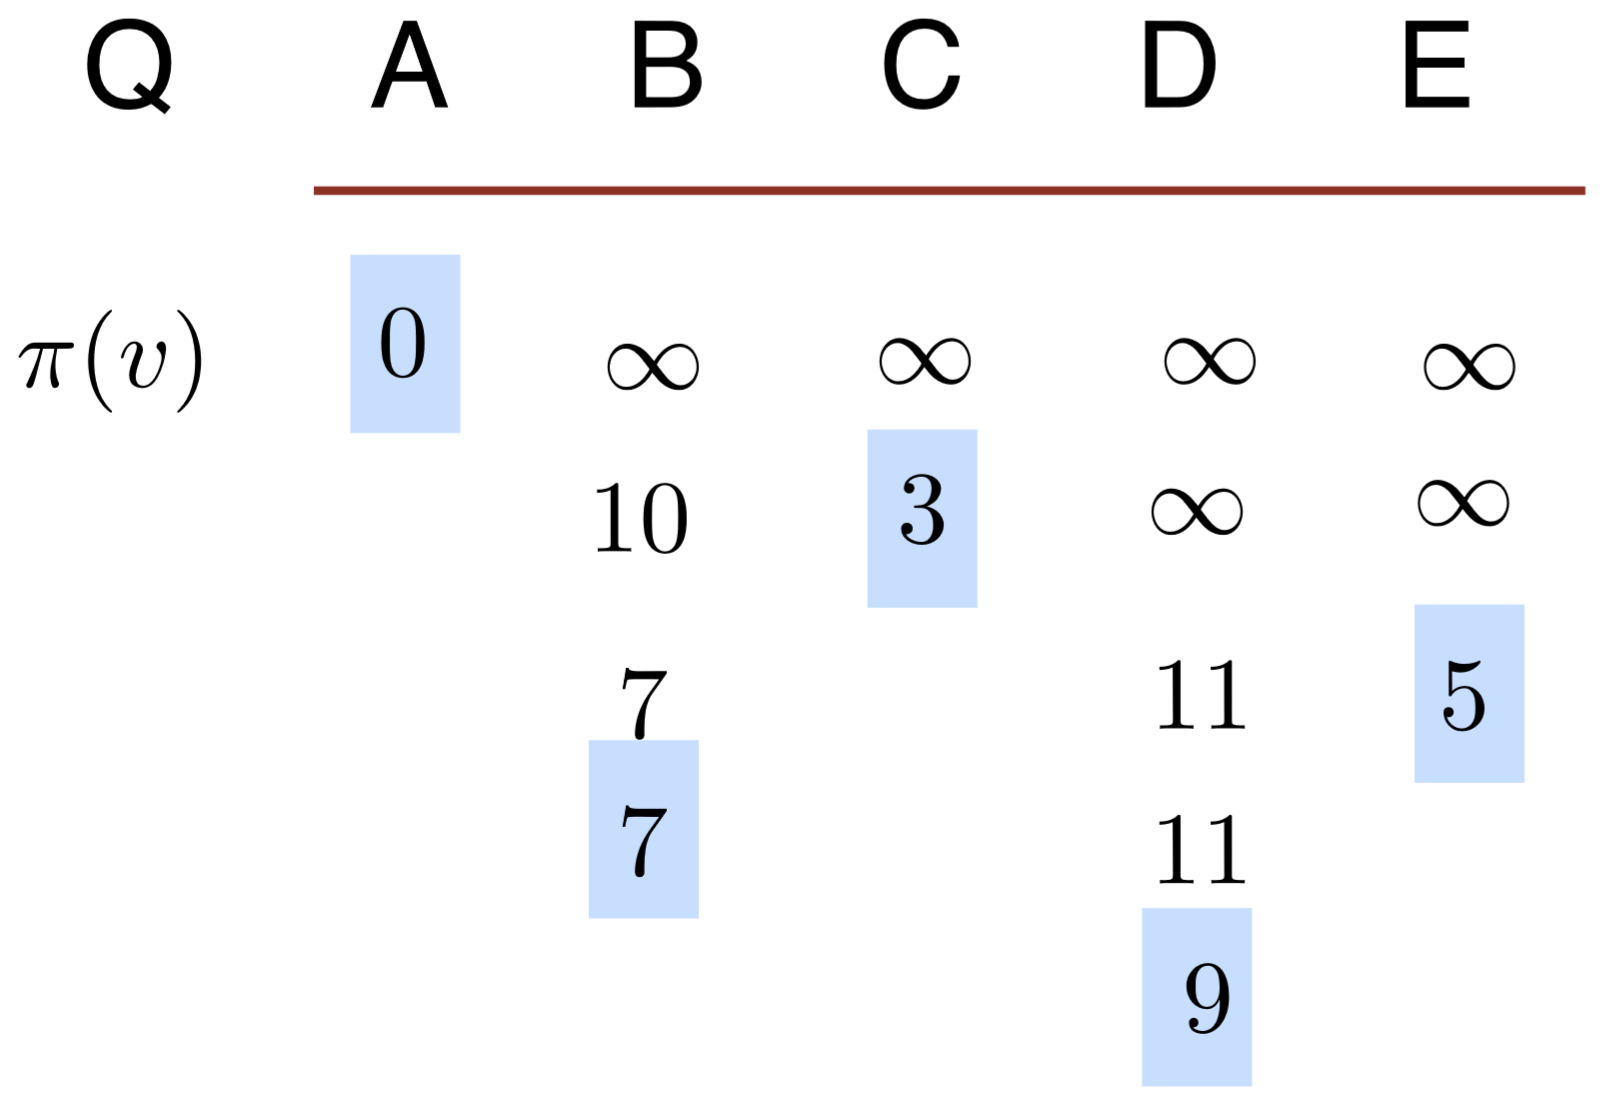
\includegraphics[width=0.45\textwidth]{./Sections/dstra/w_dist.png} % First image
    \hfill % Adds space between the images
    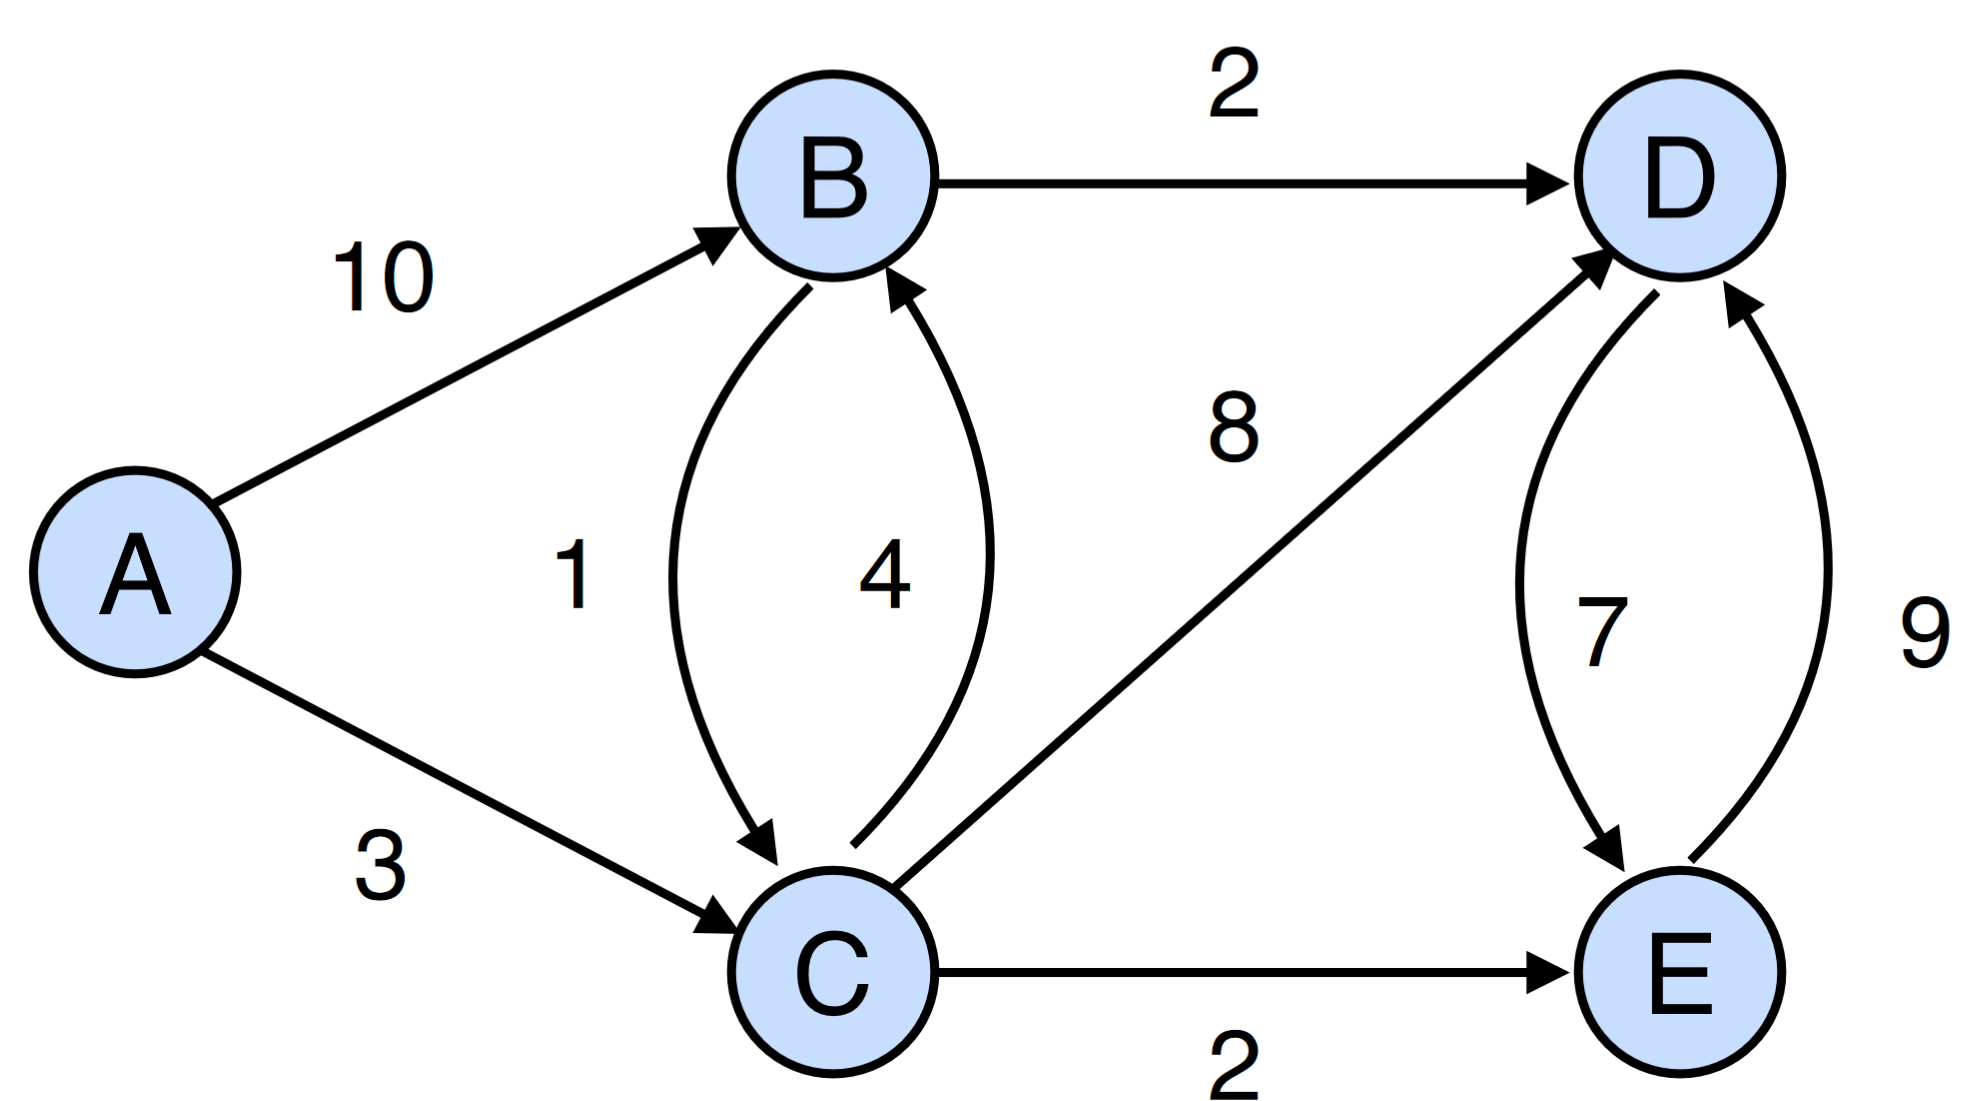
\includegraphics[width=0.45\textwidth]{./Sections/dstra/w_graph.png} % Second image
    \caption{A weighted graph and its shortest paths.}
    \label{fig:combined_figure}
\end{figure}


\noindent
In figure (\ref{fig:combined_figure}), the first row is $0$ as $s\to s$, other nodes are assumed $\infty$,i.e., undefined. Each subsequent row finds the next shortest path, while 
updating the table about information it gathers.\\
\noindent
However we have one problem with Dijkstra's algorithm, it does not work with negative weights.
\begin{theo}[Dijkstra's Algorithm and Negative Weights]
    
    Dijkstra's algorithm does not work with negative weights. This is because it assumes that the shortest path is the sum of the shortest paths. Therefore,
    if the algorithm believes it has found the shortest path, it assumes any further traversals will only increase the path length.
\end{theo}


\noindent
To illustrate the deterioration of Dijkstra's algorithm:

\begin{figure}[h]
    \begin{center}
      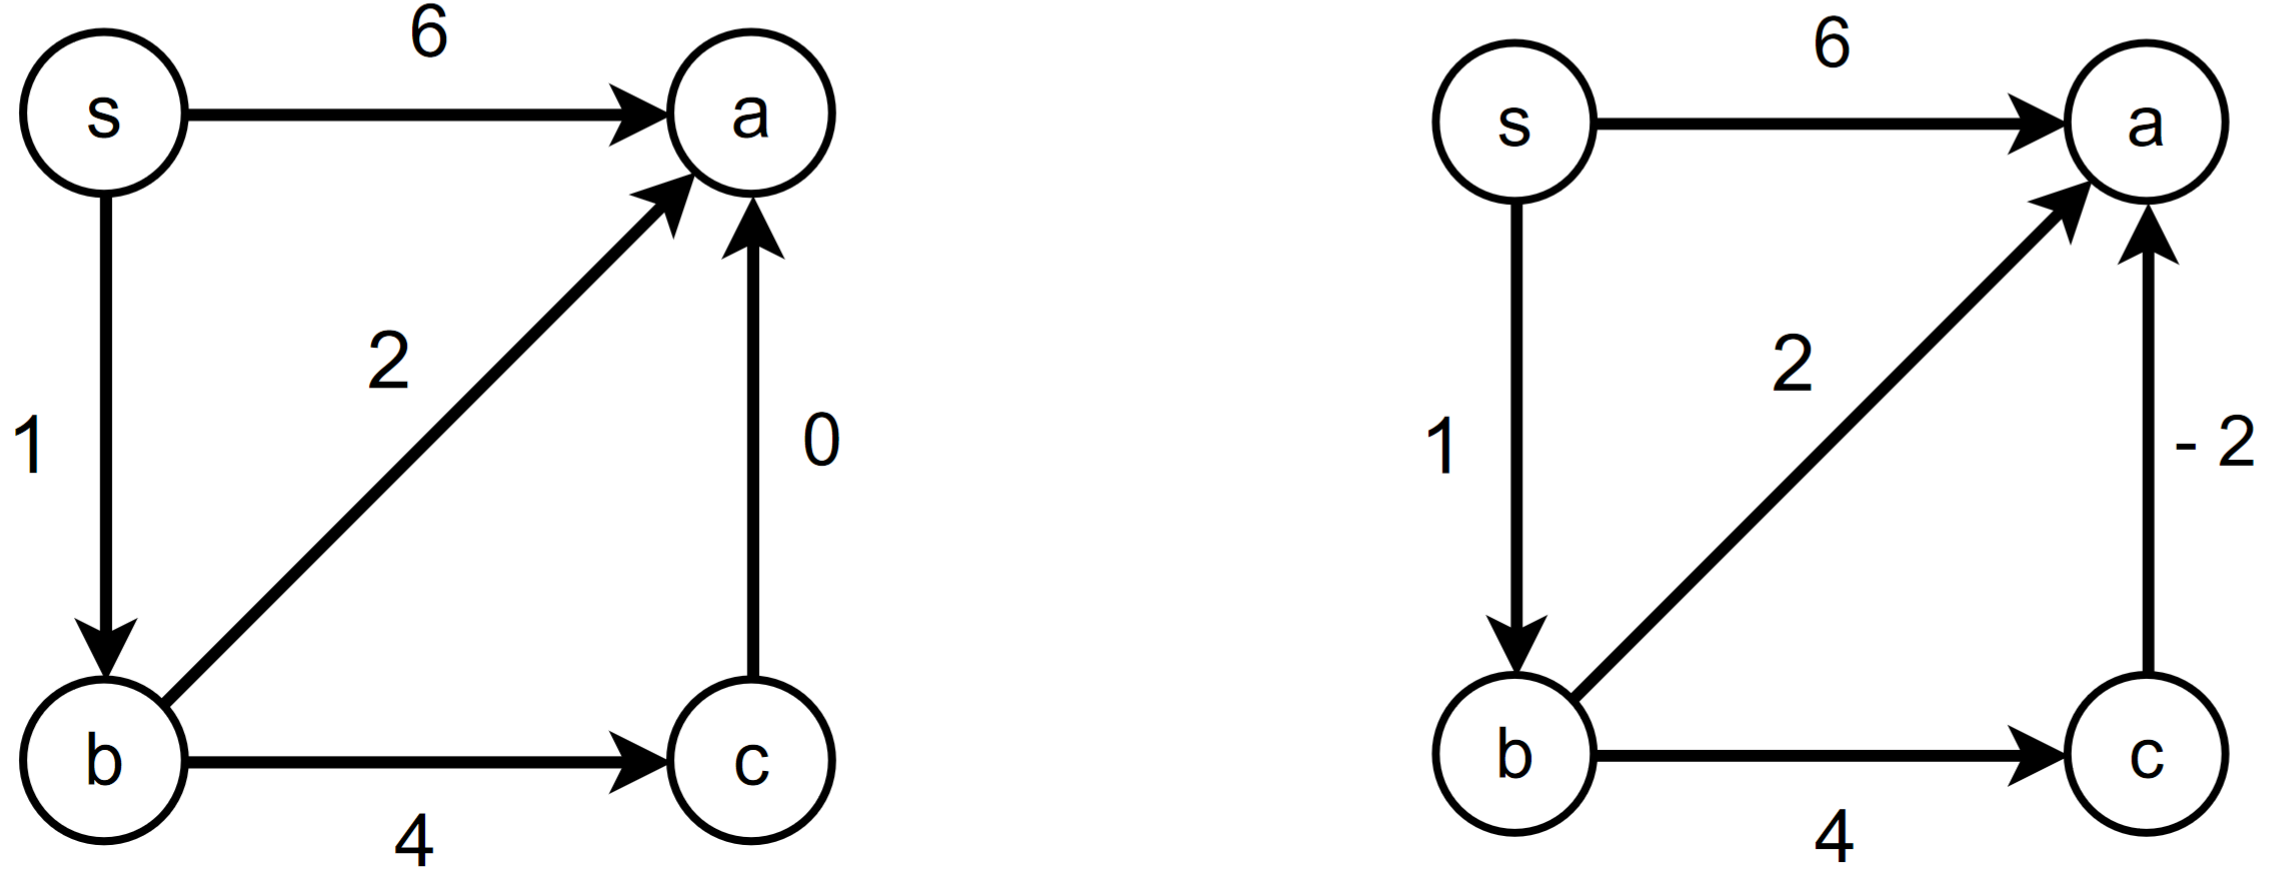
\includegraphics[height=1.5in]{./Sections/dstra/dstra_neg.png}
    \end{center}
     \caption{Shows two weighted graphs, one positive, and the other negative.}\label{fig:dstra_neg}
\end{figure}

\noindent
In Figure (\ref{fig:dstra_neg}), our negative graph will never figure out the shortest path ($s\to b\to c\to a$=1). It 
will always assume $(s\to b\to a=3)$ is the shortest path. As when it looks at $c=4$, it will think that it's 
impossible to yield any shorter of a path $3$ as anything beyond $4$ must be larger.

\newpage
\begin{Func}[Dijkstra Algorithm - \texttt{Dijkstra($G, s$)}]

    Finds the shortest path in a weighted directed graph.

    \vspace{.5em}
    \noindent
    \textbf{Input:} A graph $G = (V, E)$ with adjacency list $G[u][v] = l(u, v)$ and source node $s$.\\
    \textbf{Output:} Shortest distances $d[u]$ and parent nodes for paths.

    \begin{algorithm}[H]
        \SetAlgoLined
        \SetKwProg{Fn}{Function}{:}{\KwRet{$d, parents$}}
        \Fn{\texttt{Dijkstra($G, s$)}}{
            $\pi \gets \{\}$\tcp{hash table, current best list for $v$}
            $d \gets \{\}$\tcp{hash table, distance of $v$}
            $parents \gets \{\}$\tcp{parents in shortest path tree}
            $Q \gets \text{PQ()}$\tcp{priority queue to track minimum $\pi$}

            $\pi[s] \gets 0$\;
            $Q.\texttt{INSERT}(\langle 0, s \rangle)$\;

            \For{$v \neq s$ in $G$}{
                $\pi[v] \gets \infty$\;
                $Q.\texttt{INSERT}(\langle \pi[v], v \rangle)$\;
            }

            \While{$Q$ is not empty}{
                $\langle \pi[u], u \rangle \gets \texttt{EXTRACT-MIN}(Q)$\;
                $d[u] \gets \pi[u]$\;
                \For{$v \in G[u]$}{
                    \If{$\pi[v] > d[u] + l(u, v)$}{
                        $\texttt{DECREASE-KEY}(\langle \pi[v], v \rangle, \langle d[u] + l(u, v), v \rangle)$\;
                        $\pi[v] \gets d[u] + l(u, v)$\;
                        $parents[v] \gets u$\;
                    }
                }
            }
        }
    \end{algorithm}

    \noindent
    \textbf{Time Complexity:} $O(m\log n)$ where $m$ is the number of edges and $n$ is the number of nodes, assuming $G$ is connected $(n-1\leq m)$; Otherwise,
    $O((n+m)\log n)$.\\
    \textbf{Space Complexity:} $O(n+m)$ storing the hash-table of the graph and priority queue.
\end{Func}
